\documentclass[english,10pt,a4paper]{article}
\usepackage[utf8]{inputenc}
\usepackage[T1]{fontenc}
\usepackage{float}
\usepackage{babel}
\usepackage{amssymb}
\usepackage{graphicx}
\usepackage{hyperref}
\usepackage{mathtools}
\usepackage{amsthm}
\usepackage{nameref}
\usepackage{thmtools}
\usepackage{xcolor}
\usepackage{tikz}
\usepackage[european resistors]{circuitikz}
\hypersetup{
	pdfborder = false,
	colorlinks=true,
	linkcolor=black,
	filecolor=black,      
	urlcolor=blue,
	pdftitle={Overleaf Example},
	pdfpagemode=FullScreen,
}
\title{Stylophone\\
	\normalsize 555 timer}
\author{Kamil Chaj}
\date{2023}

\begin{document}
	\maketitle
	\tableofcontents
	\newpage
	
	\section{Introduction}
	
	\subsection{Stylophone}
	Stylophone is pocket synthesizer which uses voltage-controlled oscilator controlled with stylus which closes circuit in different position on metal keyboard on printed circuit board.
	\begin{figure}[H]
		\centering
		\includegraphics[width=0.6\textwidth]{img/Modern_Stylophone.jpg}
		\caption{Stylophone 2007}
	\end{figure}
	
	\subsection{Goal}
	Goal of this project is to recreate basic functionality of stylophone using 555 integrated circuit, make it portable by using batery as power source.
	
	\subsection{Reason}
	I wanted to build stylophone with 555 timer for some time yet I did't have sufficient knowladge and understanding of electronics to do it but now with knowladge and skills acquired during first year of my studies I can build stylophone.
	
	\subsection{History}
	Stylophone was invented by Brian Jarvis of Dubreq Studios in 1967 and initialy was produced from 1968 to 1975, but in 2007 production of stylophone was relunched. Version of stylophone from 2007 used digital electronics unlike original but in 2020 Dubreq released new analog version of stylophone which uses 555 timer integrated circuit as its heart.
	
	Number of widly known artists used stylophone in the past like The White Stripes, David Bowie or Jarvis Cocker. These days stylophone can be heard in various genres or in full stylophone covers of popular songs.
	
	\subsection{555 integrated circuit}
	555 integrated circuit, designed in 1971 by Hans Camenzind, is said to be the most popular integrated circuit ever made. 555 can be used in many configuration like: oscilators, schmit triggers, SR latches and many more.
	
	\begin{figure}[H]
		\centering
		\includegraphics[width=0.6\textwidth]{img/Signetics_NE555N.JPG}
		\caption{Signetics NE555N}
	\end{figure}
		
	Output of 555 IC can be either high or low it is dependent on state of flip-flop which is controller with 2 comparators, when voltage on pin 2(trigger) is smaller than 1/3 of supply voltage comparator sets flip-flip and output is high and stays that way until flip-flop is reset by pin 4(reset) or when voltage on pin 6(threshold) is greater than 2/3 of supply voltage.
		
	\begin{figure}[H]
		\centering
		\includegraphics[width=0.6\textwidth]{img/555_esquema.png}
		\caption{Signetics NE555 internal block diagram}
	\end{figure}
		
	\section{Design}
	\subsection{555 astable operation}
	
	555 documentation provides example circuit for astable mode of operations and formulas for properties of oscillations.
	
	\begin{equation}\label{eq:1}
		t_1 = A \cdot (R_a + R_b) C
	\end{equation}
	
	\begin{equation}\label{eq:2}
		t_2 = A \cdot R_b \space C
	\end{equation}
	
	\begin{equation}\label{eq:3}
		T = t_1 + t_2 
	\end{equation}
	
	\begin{equation}\label{eq:4}
		D = \dfrac{R_b}{R_a + 2R_b}
	\end{equation}
	
	$t_1$ - charge time, $t_2$ - discharge time, $T$ - period, $D$ - duty cycle \\
	$A = 0.693$ is constant provided in documentation
	G
	\begin{figure}[H]
		\centering
		\begin{circuitikz}[scale=1.5, transform shape, use fpu reciprocal]
	\ctikzset{resistors/scale=0.4}
	\ctikzset{capacitors/scale=0.4}
	\ctikzset{multipoles/dipchip/pin spacing = 0.5}
	\ctikzset{bipoles/oscope/waveform = square}
	
	\ctikzset{multipoles/thickness=4}
	\ctikzset{multipoles/external pins thickness=2}
	\draw (0,0) node[dipchip,
	num pins=8,
	external pins width=0.3,
	external pad fraction=4 ](C){555};
	\draw (C.pin 1) -- ++ (-0.5, 0) node[ground]{};
	\draw (C.pin 8) -- ++ (0.5, 0) node[vcc,  font=\tiny]{VCC};
	\draw (C.pin 7) to[short] ++ (0.5, 0) to[R, l_=$R_a$, font = \tiny] ++ (0, 0.7);
	\draw (C.pin 6) to[short] ++ (0.5, 0) to[R, l_=$R_b$, font = \tiny] ++ (0, 0.7);
	\draw (C.pin 6) ++ (0.5, 0) to[C, l_=$C$, font = \tiny] ++ (1, 0) node[ground]{};
	\draw (C.pin 6) ++ (0.5, 0) -- ++ (0, -1.25) -- ++ (-3.52, 0) to[short] ++ (0, 1.95) -- (C.pin 2);
	\draw (C.pin 6) ++ (0.5, 0) node[circ]{};
	\draw (C.pin 3) ++ (-1.25, 0) node[oscopeshape](O){};
	\draw (C.pin 3) ++ (-0.5, 0) node[jump crossing](X){};
	\draw (C.pin 3) -- (X.east);
	\draw (O.right) -- (X.west);
	\draw (O.center) ++ (0, 0.5) node[anchor=base, font=\tiny]{\texttt{Output}};
\end{circuitikz}
		\caption{Simplified configuration for astable mode of operation}
	\end{figure}
	
	\subsubsection{Duty cycle}
	Let's start with finding suitable component values considering duty cycle first because it is dependent on least amount of variables.
	We want duty cycle to be as close to 50\% as it is possible at least for now. According to formula \ref{eq:1} we can see that
	\begin{equation}
		\lim_{R_a \to 0} \dfrac{R_b}{R_a + 2R_b} = 0.5
	\end{equation}
	or
	\begin{equation}
		\lim_{R_b \to \infty} \dfrac{R_b}{R_a + 2R_b} = 0.5
	\end{equation}
	
	Knowing that we should choose resistance $R_a$ to be quite small and resistance $R_b$ to be much greater than $R_a$. 
	By plotting Duty cycle against resistance $R_b$ with different resistances $R_a$ we can see that in order for duty cycle to be above 48\% $R_b$ must be approximately one magnitude greater than $R_a$.
	
	\begin{figure}[H]
		\centering
		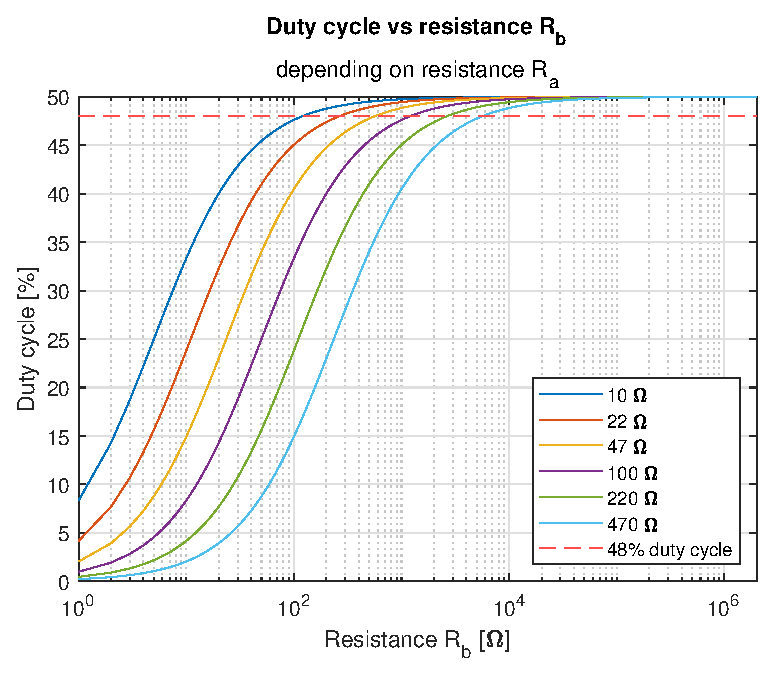
\includegraphics[width=0.7\textwidth]{img/dc_plot.eps}
	\end{figure}
	
	Before choosing $R_a$ we need to consider maximum power dissipation of the resistor and supply voltage. Resistor $R_a$ with value of 10$\Omega$ or smaller would be great to achieve 50\% duty cycle but quickly we would realized that something is smelling weird and is really hot.
	
	Power dissipation of a resistor can be calculated using formula.
	\begin{equation}
		P = \frac{V^2}{R}
	\end{equation}
	Looking first at the voltage, 555 IC requires at least 4.5V and supply voltage will not exceed 6.5V. The most common resistors used in electronic circuits have power rating of 0.25W or 1W.
	
	Knowing all restrictions we can choose the most suitable resistor $R_a$
	\begin{itemize}
		\item $R_a = 47\Omega$ for $P_{max} = 1W$
		\item $R_a = 220\Omega$ for $P_{max} = 0.25W$
	\end{itemize}
	\begin{figure}[H]
		\centering
		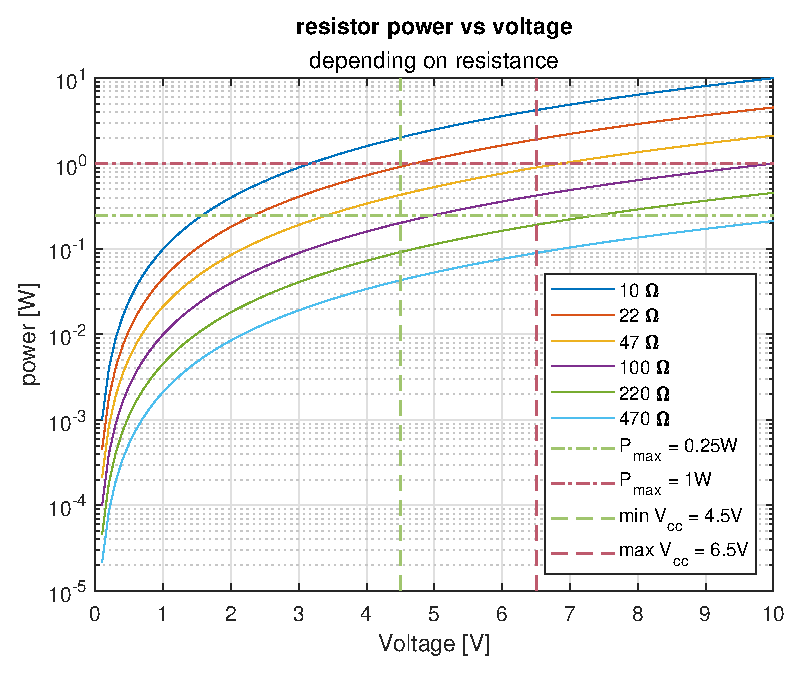
\includegraphics[width=0.7\textwidth]{img/pr_plot.eps}
	\end{figure}
	\subsubsection{Frequency range}
	Now let's consider value of capacitor C in our circuit. 
	
	\begin{figure}[H]
		\centering
		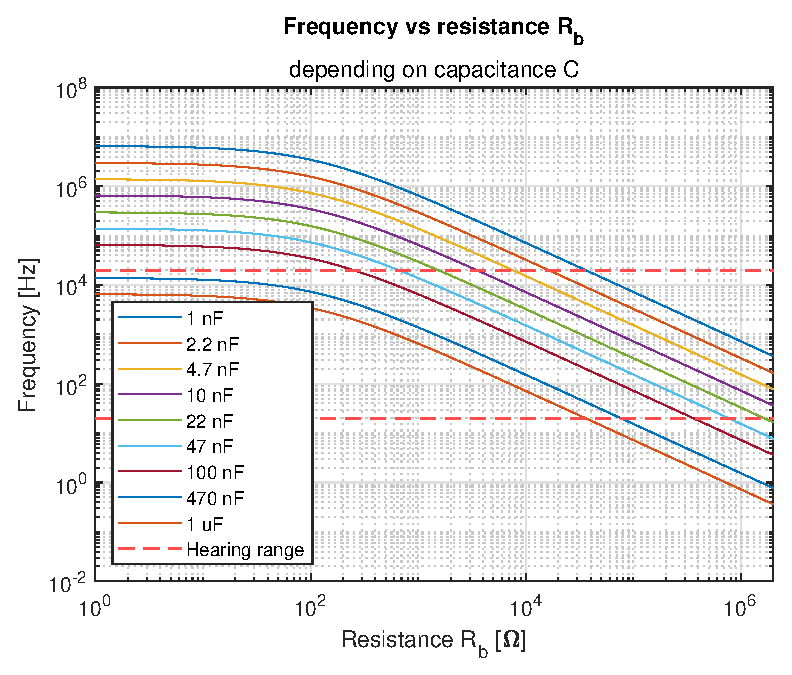
\includegraphics[width=0.7\textwidth]{img/fr_plot.eps}
	\end{figure}
	
	Stylophone's keyboard has 20 notes, one full octave, 3 notes from octave below and 5 notes above. frequency of each note can be calculated using one of following formulas
	
	\begin{equation}
		f = 2^{\frac{n}{12}} \cdot 440 \text{Hz}
	\end{equation}
	where $n$ is note number
	\begin{equation}
		f = 2^{\frac{p-69}{12}}  \cdot 440 \text{Hz}
	\end{equation}
	where $p$ is MIDI note number
	
	
	
\end{document}